\documentclass{article}

%-----------------------------------------------------------------------
% LaTeX packages
%-----------------------------------------------------------------------

\usepackage{amsfonts}
\usepackage{amsmath}
\usepackage{amsthm}
\usepackage{booktabs}
\usepackage[hmargin=1in,vmargin=1in]{geometry}
\usepackage{hyperref}
\usepackage{xspace}
\usepackage[utf8]{inputenc}
\usepackage{graphicx}
\usepackage{stmaryrd}
\usepackage{algorithm}
\usepackage[noend]{algpseudocode}
\usepackage{german}
\usepackage{xcolor}


%-----------------------------------------------------------------------
% Theorems
%-----------------------------------------------------------------------

\newtheorem{thm}{Theorem}[section]
\newtheorem{cor}[thm]{Corollary}
\newtheorem{lem}[thm]{Lemma}
\newtheorem{prop}[thm]{Proposition}
\theoremstyle{definition}
\newtheorem{defn}[thm]{Definition}
\theoremstyle{remark}
\newtheorem{rem}[thm]{Remark}

%-----------------------------------------------------------------------
% Macros
%-----------------------------------------------------------------------

\newcommand{\eg}{e.g.,\xspace}
\newcommand{\encrypt}[1]{\ensuremath{E(#1)}\xspace}
\newcommand{\decrypt}[1]{\ensuremath{D(#1)}\xspace}



%-----------------------------------------------------------------------

\begin{document}

%-----------------------------------------------------------------------
% Title
%-----------------------------------------------------------------------



\title{\begin{picture}(0,0) \put(-42,-340){\includegraphics[width=15cm]{2}} \end{picture}Solutions - Assignment 1 - Cryptography(Bachelor)}
\author{Raphael Schwegler, Marie Trojan, Fionn Edward Erickson\\
  \normalsize Matrikelnummern: 121501, 121067, 121588\ \\
  \vspace{3mm}
  \normalsize Bauhaus-Universit\"at Weimar\\
}
\pagenumbering{Roman}
\maketitle
\newpage

%-----------------------------------------------------------------------
% Content
%-----------------------------------------------------------------------

\maketitle

%___________________________Aufgabe 1___________________________________
\section*{Aufgabe 1 - Function vs. Permutation}
\subsection*{a1} Is not a function because for every element $x \in X$ should be mapped to one element of $f(x) \in Y$, however $x_2$ is mapped to two elements hence it is not a function.
\subsection*{a2} Is not a function because for every element $x \in X$ should be mapped to one element of $f(x) \in Y$ but $x_3$ does not map to any element.
\subsection*{a3} Is a general function as every $x \in X$ is mapped. It is not an injection or surjection as neither one to one or onto conditions are meet and since it is neither it is also not a bijection. 
\subsection*{a4} Is a surjection function as $x \in X$ is mapped onto a $f(x) \in Y$ and the one to one codition is meet meaning every $f(x) \in Y$ has a $x \in X$.
\subsection*{a5} Is a general funciton. Same reasoning as a3.
\subsection*{a6} Is not a function. Same reasoning as a2 except that $x_1$ is not mapped this time.
\subsection*{b}
We will break this question into its two parts, if $n>m$ and if $n<m$. First let us look at $n>m$ in which case not every $x \in X$ can be mapped to only one $f(x) \in Y$ hence it cannot be a bijection. If $n<m$ then we can map one to one or onto but not both at the same time hence it also cannot be a bijection.
\subsection*{c}
Since $f$ and $g$ are permutations over $X$ they are by definition bijective maps from $X$ to itself. We will prove that the $g(f(\cdot))$ is also bijective and thereby also a permutation over $X$.\\
If we take any arbitrary $a,b\in X$ such that $f(g(a)) = f(g(b))$. By injectivity of f we find that $g(a) = g(b)$ and by injectivity of g we find that $a=b$ hence we find that $f\circ g$ is injective. Next for every element $b\in X$ there must exist $f(g(a)) = b$ for it to be a surjection and by combiation with the proof of injection a bijection. Take the element $a=f^{-1}(g^{-1}(b))$ then  $f(g(a))=f(g(f^{-1}(g^{-1}(b))))$ simplifes to $f(g(a)) = b$ hence we have shown that it is surjective and thereby bijective.\\ 
Since a permutation is a bijection, every input is covered by a different output. That’s why g(f(x)) is also a permutation over X.
\\\\
Idea for proof comes from:\\
https://math.stackexchange.com/questions/3100050/proof-that-composition-of-two-permutations-is-again-a-permutation
\\
\subsection*{d}
A function does not have to be a bijection hence $f\circ g$ does not have to be a permutation. Let us use an example to prove this point:\\\\
If $X = \{1,2,3,4,5\}$ let us look at the following where the first row represents the input and the second row the associated mapping:\\
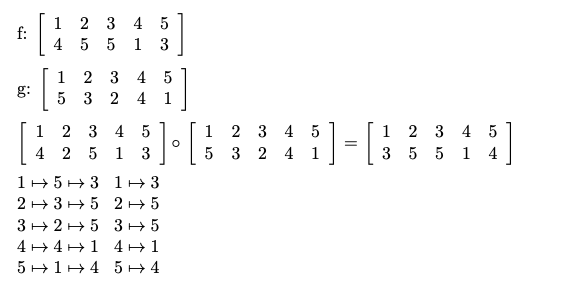
\includegraphics[width=450px]{Task1d.png}
the result is not a permutation anymore because both 2 and 3 mapped to five hence we do not meet the requirements of onto or one to one. If the function f isn’t a bijection this would always be the case because if there are at least two outputs with the same value in the function there will always be at least two values that mapped to the same values by f after the permutation.
\subsection*{f}
A permutation of the set $\{0, 1\}^n f : \{0, 1\}^n \to \{0, 1\}^n$ will keep the same Hamming weight, because the output will be all kind of variations of the input and in that way out permutation will keep the Hamming weight.
\section*{Aufgabe 2 - Complexity}
\subsection*{a}
1 hour = $20*2^{32}$\\
$20*2^{32}$ =85899345920\\\\
1 day = $24*20*2^{32}$ \\
$24*20*2^{32}$ =2061584302080\\\\
1 month(30days) = $30*24*20*2^{32}$\\
$30*24*20*2^{32}$ =61847529062400\\\\
1 year(365days) = $365*24*20*2^{32}$\\
$365*24*20*2^{32}$ =752478270259200\\
\subsection*{b}
For 64 bits we need to have $2^{64}$ iterations to check every key so assuming a average it would take Alice 24514years, 288days, 12 hours and 48minutes. For $2^{128}$ it would take more than $4,5*10^2^3$ years.

\section*{Aufgabe 3 - Two-Time Pad}
\dq d549e5020141953bb7c0a891fa624f44be42a5eb\dq contains 40 characters and \dq Send 100 Euro to Bob\dq contains 20 characters (whitespaces included), that would mean every two characters in the ciphertext is a character from the plaintext. If we use the key of the One-Time-Pad again, to encrypt \dq Send 500 Euro to Eve \dq only eight (for if seen from the plaintext) characters would change. In this case: \\
Send \colorbox{gray}{5}00 Euro to \colorbox{gray}{Eve}\\
d549e50201\colorbox{gray}{41}953bb7c0a891fa624f44be\colorbox{gray}{42a5eb}\\[2mm]
The Problem with One-Time-Pad is, that you can’t use it twice and expect it to be secure.\\
Only a few characters will change, this concludes that the Two-Time-Pad is a really bad idea since it is calles One-Time-Pad for a reason.
\section*{Aufgabe 4 - Perfect Secrecy}
\subsection*{a)}
\begin{itemize}
    \item[(a)] $Pr[M=3] = 1 - (Pr[M=0] + Pr[M=1] + Pr[M=2]) = \frac{1}{7}$
    \item[(b)] $Pr[M=3] = 1 - (Pr[M=0] + Pr[M=1] + Pr[M=2]) = \frac{1}{3}$
\end{itemize}
\subsection*{b)}
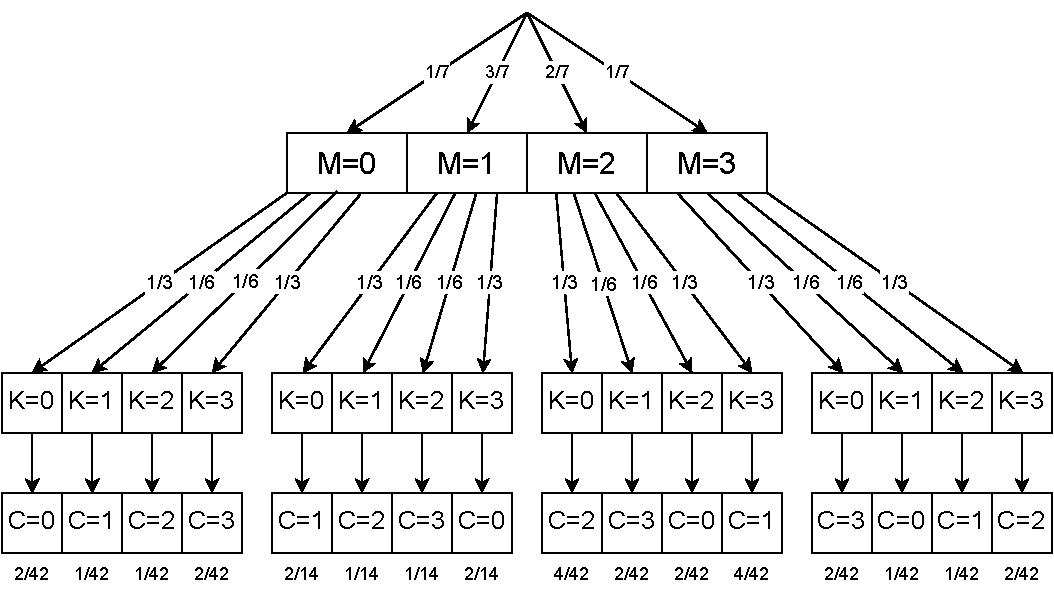
\includegraphics[scale = 1]{perfect_cipher.pdf}
\begin{itemize}
    \item[(1)]$Pr[C=0]=\frac{2}{42}+\frac{2}{14}+\frac{2}{42}+\frac{1}{42}=\frac{11}{42}$
    \item[(2)]$Pr[C=1]=\frac{1}{42}+\frac{2}{14}+\frac{4}{42}+\frac{1}{42}=\frac{12}{42}$
    \item[(3)]$Pr[C=2]=\frac{1}{42}+\frac{1}{14}+\frac{2}{42}+\frac{2}{42}=\frac{8}{42}$
    \item[(4)]$Pr[C=3]=\frac{2}{42}+\frac{1}{14}+\frac{4}{42}+\frac{2}{42}=\frac{11}{42}$
\end{itemize}
The result should be true, though $\frac{11}{42} + \frac{12}{42} + \frac{8}{42} + \frac{11}{42}=1$ 
\subsection*{c)}
To be a perfect cipher it must fulfill the following condition\\
$Pr[M=x|C=y]=Pr[M=x]$\\[2mm]
To get $Pr[M=x|C=y]$ we can use Bayes theorem $Pr[M=x|C=y]=\frac{Pr[M=x]*Pr[C=y|M=x]}{Pr[C=y]}$
Let's test this for M=0 and C=0 (also $Pr[C=y|M=x]=Pr[M=x]$):\\[2mm]
$Pr[M=0|C=0]=\frac{Pr[M=0]*Pr[C=0|M=0]}{Pr[C=0]}$\\[2mm]
$\phantom{Pr[C=0|M=0]}=\frac{Pr[M=0]*Pr[K=0]}{Pr[C=0]}$\\[2mm]
$\phantom{Pr[C=0|M=0]}=\frac{\frac{1}{7}*\frac{1}{3}}{\frac{11}{42}}=\frac{\frac{1}{21}}{\frac{11}{42}}=\frac{2}{11}\neq \frac{1}{7}$\\[2mm]
We see that $Pr[M=0|C=0]\neq Pr[M=0] $ \\[2mm]
We see this ciper is not perfekt.
\section*{Aufgabe 5 - LFSR}
\begin{itemize}
    \item[a)] The LSFR will never change if the initial state is all zeros, since zero will remain zero.
    \item[b)]\phantom{hi} \\
    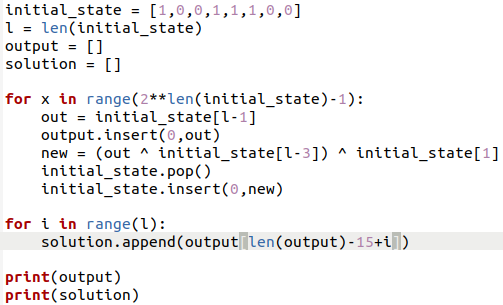
\includegraphics[scale = 0.5]{Task_5_b.png}\\
    We recieve our solution by running our LSFR in a loop for $2^n -1$ times, since it is a property of the LSFR to repeat itself.\\
    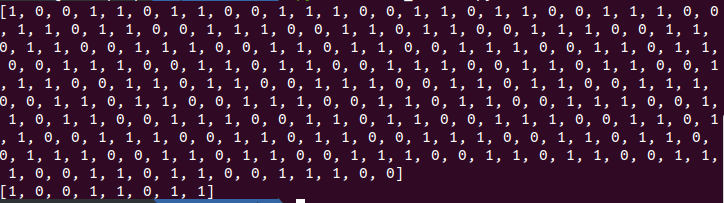
\includegraphics[scale=0.5]{Task5b_solution.png}\\
    We achieve the solution (1,1,0,0,1,1,0,1)
\end{itemize}



\end{document}

